\documentclass[../physics12.tex]{subfiles}
\graphicspath{{\subfix{../figures/}}}
\begin{document}
\chapter{Magnetism}
\section{Formulas}
Magnetic force on a moving charge: $F=qvB\sin\theta$

Magnetic force on a current carrying wire: $F=BIl\sin\theta$

Magnetic moment of a current carrying coil of N turns: $\mu = NIA$

Torque on a current carrying coil: $\tau = \mu B \sin\theta$

Radius of uniform circular motion of a charged particle in a magnetic field: $r=\frac{mv}{qB}$

Magnetic field of a long straight wire: $B=\frac{\mu_0 I}{2\pi r}$

Ampere's Law: $\sum B_{\parallel}\Delta l = \mu_0 I$

Magnetic force between two parallel wires: $\frac{F}{l} = \frac{\mu_0 I_1 I_2}{2\pi d}$

Magnetic field at the center of a circular coil: $B = \frac{\mu_0 I}{2r}$

Magnetic field inside a solenoid: $B = \mu_0 nI = \mu_0 NI/l$

\section{Electron Orbiting Hydrogen Atom Problem}
In Niels Bohr's 1913 model of the hydrogen atom, and electron circles the proton at a distance of $8.24\times 10^{-11}$ m with a speed of $9.16\times 10^5$ m/s.
The permeability of free space is $1.25664\times 10^{-6}$ T$\cdot$ m/A.

Compute the magnetic field strength that this motion produces at the location of the proton. Answer in units of T.

\section{Three Parallel Wires Problem}
Three very long wires are strung parallel to each other as shown in the figure below. Each wire is at a distance 31 cm from the other two, and each wire carries a current of 
magnitude $I=3.3$ A in the directions shown in the figure.
\begin{center}
    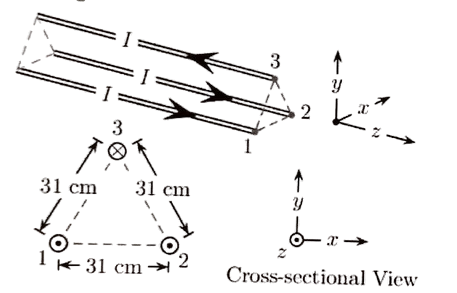
\includegraphics[width=0.5\textwidth]{11.2.PNG}
\end{center}
Find the magnitude of the net force per unit length exerted on the upper wire (wire 3) by the other two wires. Answer in units of N/m.

\section{Energy of Undeflected Electron Problem}
The charge on an electron is $1.60218\times 10^{-19}$ C and its mass is $9.10939\times 10^{-31}$ kg. 

What is the kinetic energy of an electron that passes undeviated through perpendicular electric and magnetic fields if $E=0.23$ kV/m and $B=1.5$ mT? Answer in units of eV.

\section{Torque on Circular Loop Problem}
A circular loop of radius 3.82 cm contains 64 turns of tightly wound wire. 

If the current in the windings is 0.328 A and a constant magnetic field of 0.384 T makes an angle of $66\degree$ with a vector perpendicular with the loop, what torque acts on the loop? Answer in units of N$\cdot$m.

\section{Dropped Steel Beam Problem}
A 8.97 m long steel beam is accidentally dropped by a construction crane from a height of 12.3 m. The horizontal component of the Earth's magnetic field over the region is 23.3 $\mu$T. The acceleration of gravity is 9.8 m/s$^2$.

What is the induced emf in the beam just before impact with the Earth, assuming its long dimension remains in a horizontal plane, oriented perpendicularly to the horizontal 
component of the Earth's magnetic field? Answer in units of mV.

\section{Right Hand Rule Problems}
A negatively charged particle moving at $45\degree$ angles to both the $x$-axis and $y$-axis enters a magnetic field (pointing into of the page), as shown. 
$\hat{i}$ is in the $x$-direction, $\hat{j}$ is in the $y$-direction, and $\hat{k}$ is in the $z$-direction. 
\begin{center}
    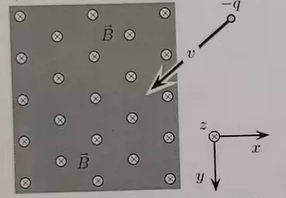
\includegraphics[width=0.5\textwidth]{11.1.PNG}
\end{center}
What is the initial direction of deflection?

\end{document}